\chapter{Результаты расчета}
\label{Chapter3}
\setlength{\parindent}{0pt}

\section{Исходные данные}
$P_\text{в}=10^5$ \si{\text{Па}} - внешнее давление в начальный момент времени \\
$\rho=1.2041$ \si{\text{кг}\per\text{м}\cubed} - плотность воздуха \\
$F_\text{a}=0.5$ \si{\text{м}\squared} - площадь выходного сечения сопла \\
$P_\text{а}=0.8\cdot 10^5$ \si{\text{Па}} - давление в выходном сечении сопла в начальный момент времени \\
$R=287$\si[per-mode = fraction]{\text{Дж}\per(\text{моль}.\text{К})} - универсальная газовая постоянная \\
$T=293$ \si{\text{К}} - температура торможения \\
$\varGamma=1.4$ - показатель адиабаты \\
$M=3$ - число Маха \\
$d_\text{а}=0.8$ \si{\text{м}} - диаметр выходного сечения сопла \\
$d_\text{к}=1$ \si{\text{м}} - диаметр кормы \\
$d_\text{тр}=1.2$ \si{\text{м}} - диаметр трубы \\
$\alpha=10$ \si{\degree} - угол полураствора сопла \\
$x=10$ \si{\text{м}} - длина эжектирующего участка \\

\section{Изменения основных величин}

\begin{figure}[H]
    \label{fig:ExternalPressure}
    \centering
    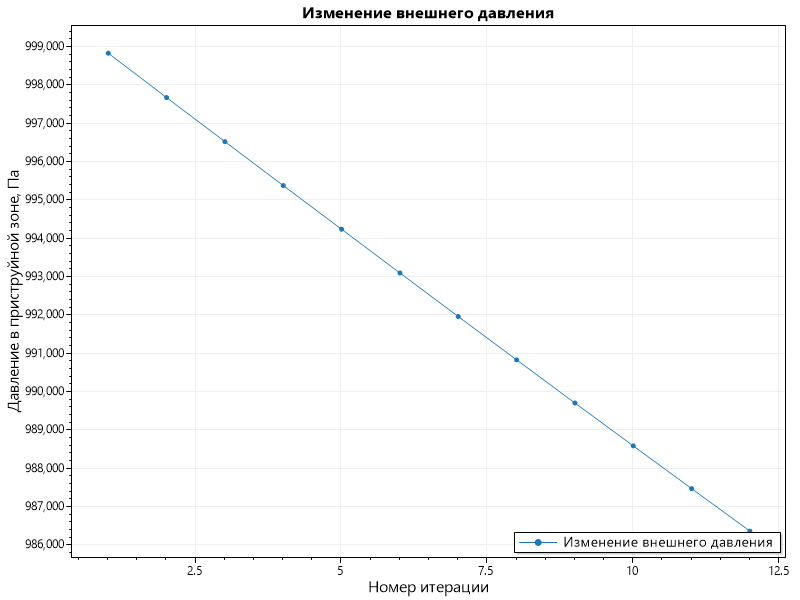
\includegraphics[width=13cm]{Figures/Pext.png}
    \caption{Изменение давления в приструйной зоне}
\end{figure}

\begin{figure}[H]
    \label{fig:EjectionLosses}
    \centering
    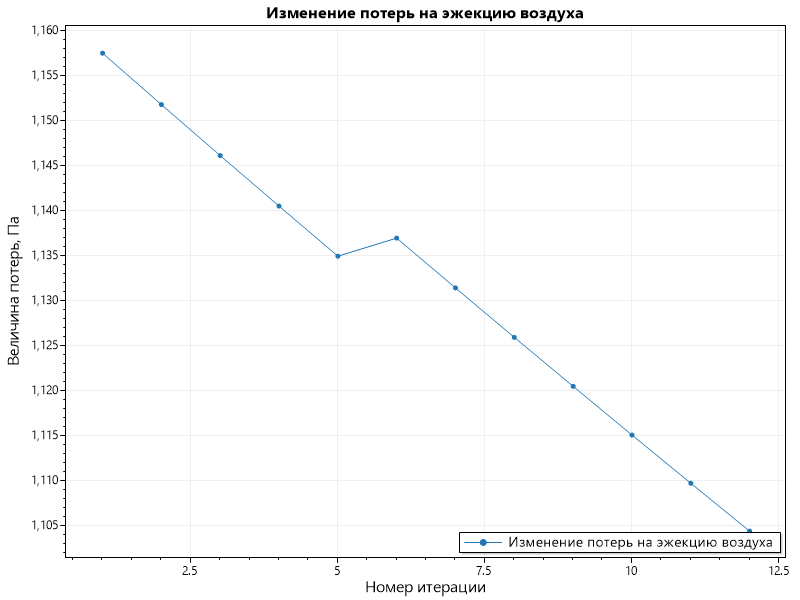
\includegraphics[width=13cm]{Figures/Hej.png}
    \caption{Изменение потерь на эжекцию приструйсного воздуха}
\end{figure}

\begin{figure}[H]
    \label{fig:LocalLosses}
    \centering
    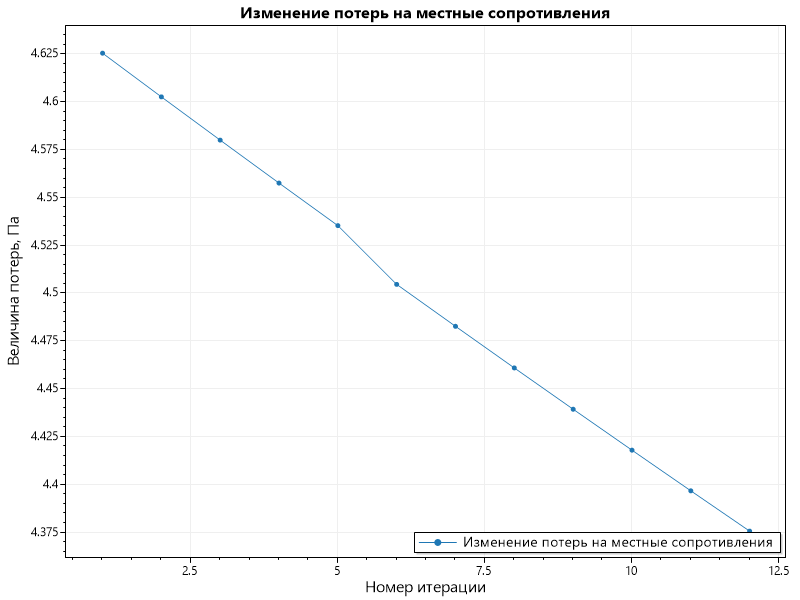
\includegraphics[width=13cm]{Figures/Hl.png}
    \caption{Изменение потерь на местных сопротивлениях в зазоре}
\end{figure}

\begin{figure}[H]
    \label{fig:FluidStructure}
    \centering
    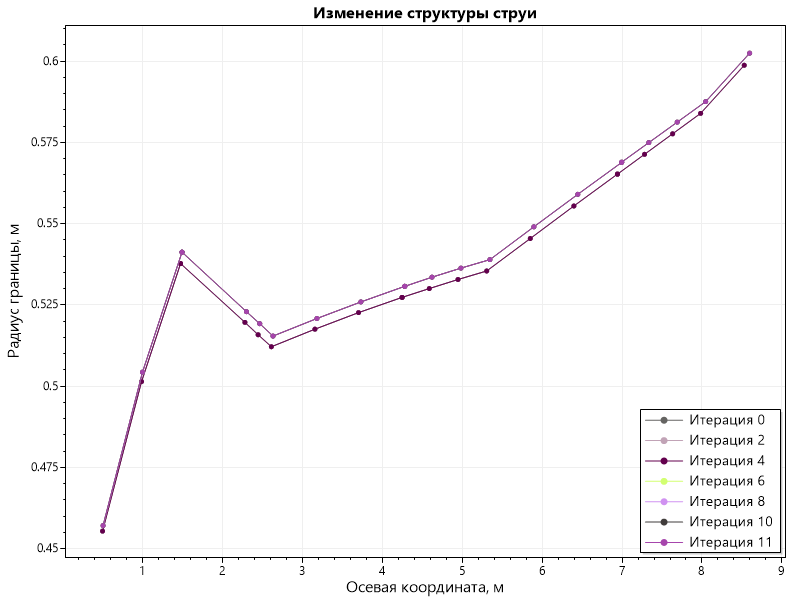
\includegraphics[width=13cm]{Figures/FluidStruct.png}
    \caption{Изменение структуры струи}
\end{figure}
